	Hacemos una validación cruzada para una muestra de data de 906130 sesiones de usuarios para probar como se comporta con {cross validation}.
	
	
	\begin{table}[tb]
		\centering
		\label{my-label}
				\resizebox{0.9\textwidth}{!}{
		\begin{tabular}{ccccc}
			\textbf{pruebas} & \textbf{entrenamiento} & \textbf{accuracy} & \textbf{nodos} & \textbf{niveles} \\
			990              & 10                     & 0,425190839694656 & 38             & 5                \\
			950              & 50                     & 0,44595041322314  & 95             & 5                \\
			900              & 100                    & 0,49089861751152  & 132            & 5                \\
			800              & 200                    & 0,567230538922155 & 181            & 5                \\
			700              & 300                    & 0,606837606837608 & 208            & 5                \\
			600              & 400                    & 0,649253731343282 & 241            & 5                \\
			500              & 520                    & 0,714285714285715 & 264            & 5               
		\end{tabular}
	}
			\caption{Tabla resumen experimento 6}
	\end{table}
	
	
	
	
	\begin{table}[tb]
		\centering
		\caption{Tabla resumen para sesiones mayores de 100000 sesiones}
		\label{my-label}
		\resizebox{.8\textwidth}{!}{
		\begin{tabular}{ccccc}
			\textbf{pruebas} & \textbf{entrenamiento}  & \textbf{accuracy} & \textbf{nodos} & \textbf{niveles} \\
			990              & 100                     & 0,299674371114825  & 61            & 4               \\
			950              & 200                     & 0,449237667712101  & 108           & 5               \\
			900              & 1000                    & 0,56519572924979   & 242           & 5               \\
			800              & 2500                    & 0,689237667712101  & 336           & 5               

		\end{tabular}
		}
	\end{table}
	
	
	
	\begin{figure}[h] 
		\centering
			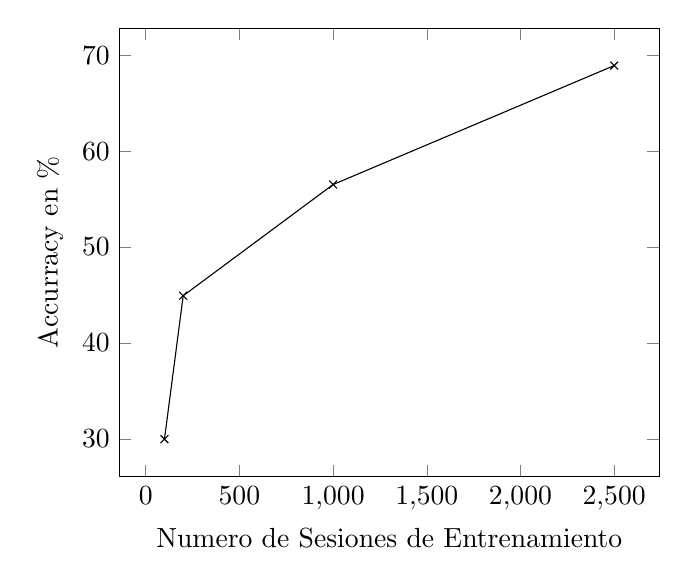
\begin{tikzpicture}
			\begin{axis}[
			xlabel= Numero de Sesiones de Entrenamiento,
			ylabel=Accurracy en \% ]
			\addplot[color=black,mark=x] coordinates {
				(100, 29.9674371114825)
				(200, 44.9237667712101)
				(1000, 56.519572924979)
				(2500, 68.9237667712101)	
			};
			\end{axis}
			\end{tikzpicture}
		\caption{Gráfico de Accuracy vs sesiones de entrenamiento para una cota superior de 5 símbolos}
		\label{fig:sim}
	\end{figure}
	
	\begin{table}[]
		\centering

		\label{my-label}
		\resizebox{1\textwidth}{!}{
		\begin{tabular}{lccccccccccccccccc}
			\textbf{símbolo}                                                                  & A                         & B                         & C                         & D                         & E                        & F                         & G                        & H                         & I                         & J                        & K                        & L                         & M                         & N                         & O                        & P                       & Q                       \\
			\textbf{\begin{tabular}[c]{@{}l@{}}frecuencia \\ 1000 sesiones\end{tabular}}      & 31086                     & 14262                     & 5483                      & 15458                     & 12713                    & 7717                      & 8255                     & 4155                      & 2381                      & 9697                     & 1974                     & 9584                      & 1871                      & 12795                     & 3935                     & 11735                   & 506                     \\
			\textbf{\begin{tabular}[c]{@{}l@{}}frecuencia \\ 100.000\\ sesiones\end{tabular}} & \multicolumn{1}{l}{43173} & \multicolumn{1}{l}{20251} & \multicolumn{1}{l}{15093} & \multicolumn{1}{l}{12790} & \multicolumn{1}{l}{1458} & \multicolumn{1}{l}{26517} & \multicolumn{1}{l}{4154} & \multicolumn{1}{l}{14517} & \multicolumn{1}{l}{12262} & \multicolumn{1}{l}{4163} & \multicolumn{1}{l}{4658} & \multicolumn{1}{l}{13180} & \multicolumn{1}{l}{14021} & \multicolumn{1}{l}{15779} & \multicolumn{1}{l}{2498} & \multicolumn{1}{l}{125} & \multicolumn{1}{l}{559}
		\end{tabular}
		}
		\caption{Tabla de frecuencia de símbolos para $1.000$ sesiones y $100.000$ }
	\end{table}
	
	